%-*- coding:utf-8 -*-

\begin{frame}[t,fragile]{ツリー法}
  \begin{itemize}
    %\setlength{\itemsep}{1em}
  \item 遠くのものをまとめて扱う
  \item 空間をメッシュで8等分(2次元の場合は4等分)していく
    \begin{center}
      \resizebox{!}{.4\textheight}{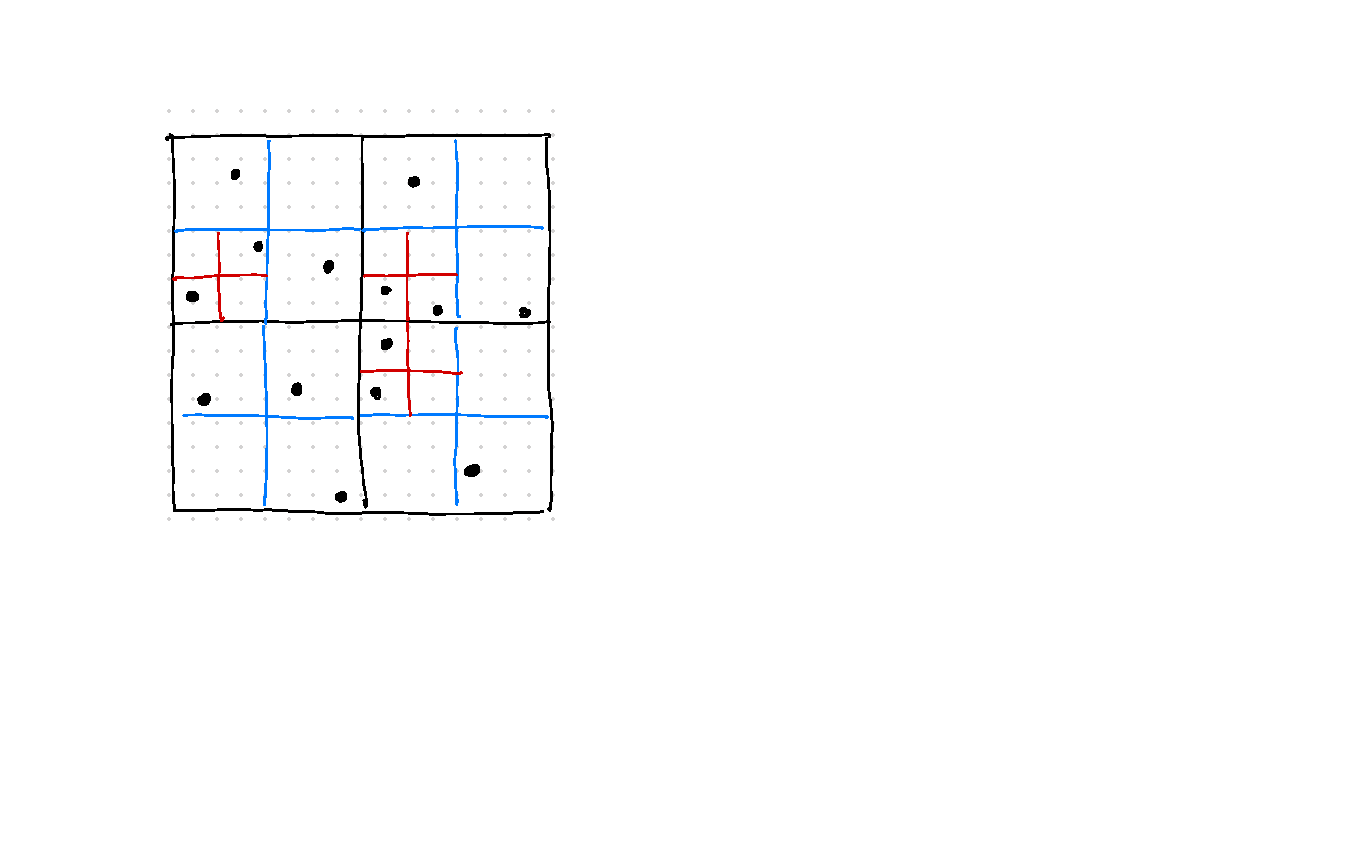
\includegraphics{image/tree-1.pdf}}
      \resizebox{!}{.4\textheight}{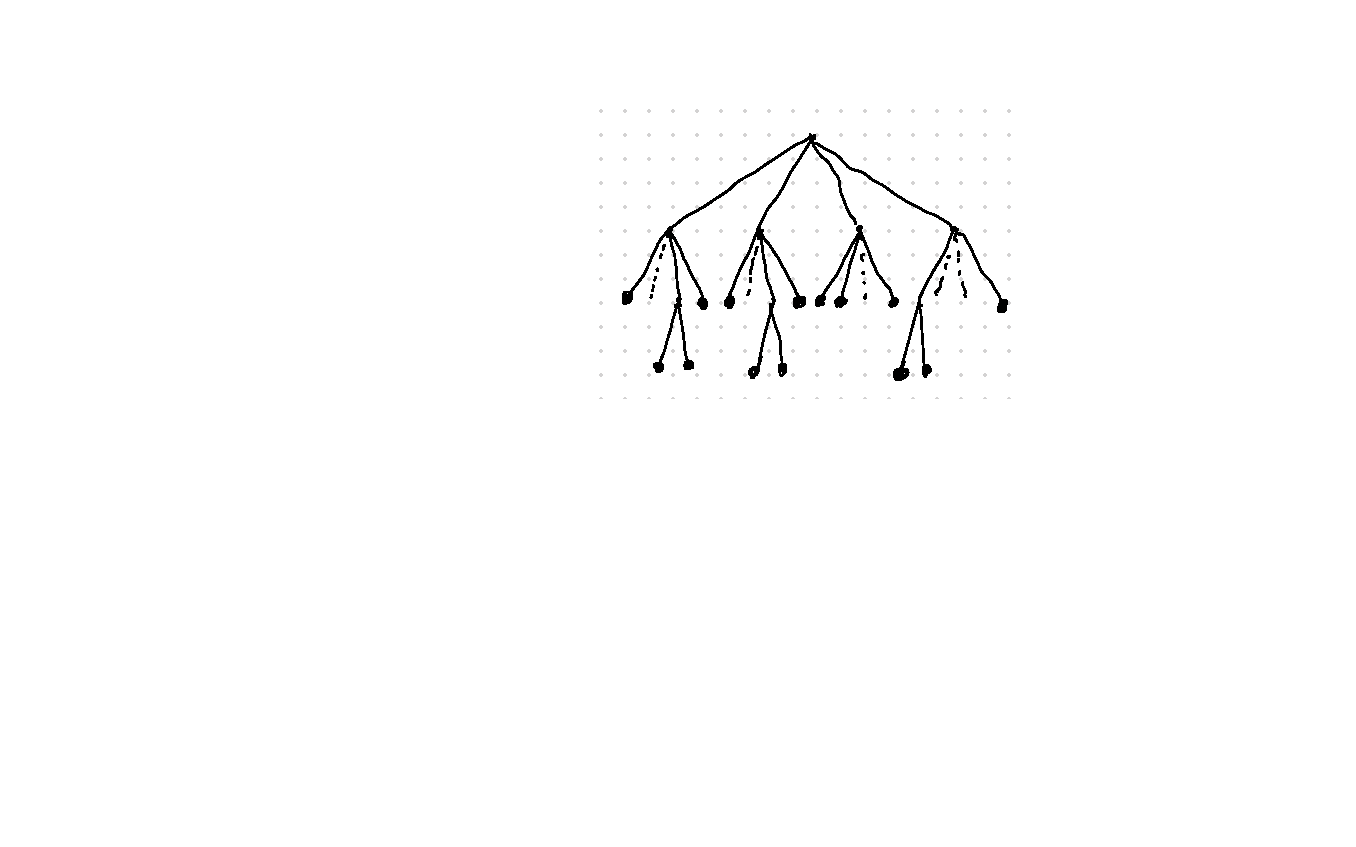
\includegraphics{image/tree-2.pdf}}
    \end{center}
    \begin{itemize}
    \item それぞれのメッシュに粒子が1個あるいは0個となるまで
    \item 全体が8分木(2次元の場合は4分木)で表現される
    \item ツリー構造の下から順番に重心と総質量を計算しておく
    \end{itemize}
  \end{itemize}
\end{frame}

